\documentclass[12pt, a4paper, substylefile = spbu.rtx]{disser}
\usepackage[utf8]{inputenc}
\usepackage[left=2cm,right=1.5cm,top=2cm,bottom=2cm]{geometry}
\usepackage[english,russian]{babel}
%\usepackage[OT1]{fontenc}
\usepackage{amsmath}
\usepackage{amssymb}
\usepackage{chngcntr}
\usepackage{amsthm}
\usepackage{wasysym}
\usepackage{isotope}
\usepackage{hyperref}
\usepackage{indentfirst}
\usepackage[shortlabels]{enumitem}
\usepackage{cmap}
\usepackage{floatrow}
\usepackage{nicefrac}
\usepackage[all]{xy}
\newcommand*{\mybibstyle}{ugost2008s}
\linespread{1,3}
\usepackage{float}
\restylefloat{table}
\usepackage{framed}
\usepackage{lipsum}
\usepackage{algorithm,algorithmic}
\usepackage{algpseudocode}
\usepackage{tikz}
\usepackage{pgfplots}
\usepackage{setspace}

\usepackage{mathrsfs}
\usetikzlibrary{arrows}

%\usepackage{theorem}
\usepackage{amsthm}
\theoremstyle{definition}   
\newtheorem{defn}{Определение}
\newtheorem{theorems}{Теорема}
\newtheorem{zam}{Замечание}

\DeclareMathOperator{\Ptr}{Ptr}
\DeclareMathOperator{\argmax}{argmax}
\DeclareMathOperator{\okras}{o}



\usepackage{graphicx} 
\graphicspath{{pictures/}} 
\DeclareGraphicsExtensions{.pdf}
\DeclareGraphicsExtensions{.png}
\DeclareGraphicsExtensions{.jpg}

\usepackage{wrapfig}

\usepackage{fancyhdr}

\ifx\pdfoutput\undefined
\usepackage{graphicx}
\else
\usepackage[pdftex]{graphicx}
\fi
\floatsetup[table]{capposition=top}

\usepackage{sectsty}
\usepackage{color}
\usepackage{listings}
\definecolor{dkgreen}{rgb}{0,0.6,0}
\definecolor{gray}{rgb}{0.5,0.5,0.5}
\definecolor{mauve}{rgb}{0.58,0,0.82}
\lstset{ %
	language=R,                % Язык программирования 
	numbers=left,                   % С какой стороны нумеровать
	stepnumber=1,                   % Шаг между линиями. Если 1, то будет пронумерована каждая строка 
	numbersep=5pt,                  
	showspaces=false,               
	showstringspaces=false,         
	showtabs=false,                
	tabsize=2,                       % Tab - 2 пробела
	breaklines=true,                 % Автоматический перенос строк
	breakatwhitespace=true,          % Переносить строки по словам
}
\allsectionsfont{\centering}
\setcounter{tocdepth}{4}
\begin{document}

	\institution{%
		Санкт-Петербургский государственный университет \\
		Прикладная математика и информатика \\
		Статистическое моделирование
	}
	
	\title{Конспект}
	
	% Тема
	\topic{\normalfont\scshape%
		Тематическое моделирование}
	
	% Автор
	\author{Калина Екатерина, Зенкова Наталья, Балагуров Владимир}
	
	%% Scientific Advisor
%	\sa       {П.\,В.~Шпилев}
%	\sastatus {к.ф.-м.н., доцент}

	
	% Город и год
	\city{Санкт-Петербург}
	\date{\number\year}
	
	\maketitle
	
	%%
	%% Titlepage in English
	%%
	%
	\institution{%
		Saint Petersburg State University \\
		Applied Mathematics and Computer Science \\
		Computational Stochastics and Statistical Models
	}
	%
	\title{Graduation Project}
	%
	%% Topic
	\topic{\normalfont\scshape %
		A simulation approach to the solution of strategic games with incomplete information}
	%
	%% Author
	\author{Bakshinskaia Ekaterina} % Full Name
	%
	%% Scientific Advisor
	\sa       {P.\,V.~Shpilev}
	\sastatus {Associate professor}
	%
	%% Reviewer
	%\rev      {N.\,P.~Alekseeva}
	%\revstatus{Associate professor}
	%
	%% City & Year
	\city{Saint Petersburg}
	\date{\number\year}
	%
%	\maketitle[en]
	
       
    \tableofcontents
    
 \definecolor{ududff}{rgb}{0.30196078431372547,0.30196078431372547,1}
 \definecolor{cqcqcq}{rgb}{0.7529411764705882,0.7529411764705882,0.7529411764705882}   

   
   \section{Введение}
   
   Тематическое моделирование (topic modeling) --- одно из современных приложений машинного обучения к анализу текстов. Тематическая модель коллекции текстовых документов определяет, к каким темам относится каждый документ и какие слова (термины) образуют каждую тему.
   
Вероятностная тематическая модель (ВТМ) описывает каждую тему дискретным распределением на множестве терминов, каждый документ --- дискретным распределением на множестве тем. Предполагается, что коллекция документов --- это последовательность терминов, выбранных случайно и независимо из смеси таких распределений, и ставится задача восстановления компонент смеси по выборке.

Поскольку документ или термин может относиться одновременно ко многим темам с различными вероятностями, говорят, что ВТМ осуществляет «мягкую» кластеризацию документов и терминов по кластерам-темам. Тем самым решаются проблемы синонимии и омонимии терминов, возникающие при обычной «жёсткой» кластеризации. Синонимы, часто употребляющиеся в схожих контекстах, с большой вероятностью попадают в одну тему. Омонимы, употребляющиеся в разных контекстах, распределяются между несколькими темами соответственно частоте употребления.

Некоторые приложения тематического моделирования:

\begin{itemize} 
\item разведочный поиск в электронных библиотеках;
\item поиск тематического контента в соцсетях;
\item детектирование и трекинг новостных сюжетов;
\item мультимодальный поиск текстов и изображений;
\item анализ банковских транзакционных данных.
\end{itemize}

\section{Вероятностная модель коллекции документов} 
   
   \subsection{Постановка задачи}
    
   Пусть $D$ --- множество (коллекция) текстовых документов, $W$ --- множество (словарь) всех употребляемых в них терминов (слов или словосочетаний). Каждый документ $d\in D$ представляет собой последовательность $n_d$ терминов $(w_1, . . . , w_n_d)$ из словаря $W$. Термин может повторяться в документе много раз.
   
   Предполагается, что существует конечное множество тем $T$, и каждое употребление термина $w$ в каждом документе $d$ связано с некоторой темой $t\in T$, которая не известна. Коллекция --- это i.i.d выборка $(d_i,w_i,t_i)^n_{i=1}\sim p(d,w,t)$, заданная на конечном множестве $D\times W\times T$. 

Документы $d\in D$ и термины $w\in W$ являются \textit{наблюдаемыми переменными}, тема $t\in T$ является \textit{латентной (скрытой) переменной}.
   
   Таким образом,
   
   \begin{itemize} 
\item Тема --- условное распределение на множестве терминов,
$p(w|t)$ --- вероятность термина $w$ в теме $t$
\item Тематический профиль документа --- условное распределение
$p(t|d)$ --- вероятность темы $t$ в документе $d$
\end{itemize}
   
   \textbf{Задача тематического моделирования.} Построить тематическую модель коллекции документов $D$ --- значит найти множество тем $T$, распределения $p(w|t)$ для всех тем $t\in T $ и распределения $p(t|d)$ для всех документов $d\in D$. 

Найденные распределения используются затем для решения прикладных задач. Распределение $p(t|d)$ является удобным признаковым описанием документа в задачах информационного поиска, классификации и категоризации документов.

  \renewcommand{\algorithmicrequire}{\textbf{Input:}}
\renewcommand{\algorithmicensure}{\textbf{Output:}}

   
  \subsection{Гипотезы и предположения} 
   
   \textbf{Гипотеза независимости.} Гипотеза о независимости элементов выборки эквивалентна предположению,
что порядок терминов в документах не важен для выявления тематики, то есть тематику документа можно узнать даже после произвольной перестановки терминов, хотя для человека такой текст теряет смысл. Это предположение называют гипотезой «мешка слов» (bag of words). Порядок документов в коллекции также не имеет значения; это предположение называют гипотезой «мешка документов».

Приняв гипотезу «мешка слов», можно перейти к более компактному представлению документа как подмножества $d\subset W$, в котором каждому элементу $w\in d$ поставлено в соответствие число $n_{dw}$ вхождений термина $w$ в документ $d$.
   
   \textbf{Гипотеза условной независимости.} Будем полагать, что появление слов $w$ в документе $d$, относящихся к теме $t$, описывается общим для всей коллекции распределением $p(w |t)$ и не зависит от документа $d$. Это предположение, называемое гипотезой условной независимости, допускает три эквивалентных представления:
   
   \begin{equation*}
\begin{gathered}
   p(w|d,t)=p(w|t)\\p(d|w,t)=p(d|t)\\ p(d,w|t)=p(d|t)p(w|t)
   \end{gathered}
\end{equation}
   
   \textbf{Гипотеза разреженности.} Естественно предполагать, что каждый документ $d$ и каждый термин $w$ связан с небольшим числом тем $t$. В таком случае значительная часть вероятностей $p(t| d)$ и $p(w |t)$ должна обращаться в нуль.
   
   Если документ относится к большому числу тем (например, энциклопедия, журнал, сборник статей), то в задачах тематического поиска или классификации документов его имеет смысл разбивать на части, более однородные по тематике.


Если термин относится к большому числу тем, то, скорее всего, это общеупотребительное слово (стоп-слово), бесполезное для определения тематики.
   
   Алгоритмы, в которых нулевые значения не хранятся, намного эффективнее по памяти и по скорости. Поэтому для больших коллекций разреженность должна учитываться обязательно.
   
   
   
   \subsection{Предварительная обработка документов} 
   
   \textit{Мотивация:} К предварительной обработке текстов прибегают для упрощения модели. 

   
      \begin{itemize} 
\item \textbf{Лемматизация} --- это приведение каждого слова в документе к его нормальной форме. При построении тематической модели нет смысла различать формы (склонения, спряжения) одного и того же слова. Это приведёт к неоправданному разрастанию словаря, дроблению статистики, увеличению ресурсоёмкости и снижению качества модели.

Разработка хорошего лемматизатора (lemmatizer) требует составления грамматического словаря со всеми формами слов, либо аккуратной формализации правил языка со всеми исключениями, что является \textit{трудоёмким проектом}. Известные лемматизаторы совершенствуются постепенно. Их недостатком является
неполнота словарей, особенно по части специальной терминологии и неологизмов, которые во многих приложениях как раз и представляют наибольший интерес.

 \item \textbf{Стемминг} --- это более простая технология, которая состоит в отбрасывании изменяемых частей слов, главным образом, окончаний. Она не требует хранения словаря всех слов и основана на правилах морфологии языка. Недостатком стемминга является \textit{большее число ошибок}. Стемминг хорошо подходит для английского языка, но хуже подходит для русского

\item \textbf{Уменьшение словаря}:
  
   \begin{itemize} 
\item $1000,\;5,\;23\to \$number;\;\;(5+3),\;\frac12ww^T+C\to\$formula$
\item \textbf{Отбрасывание стоп-слов}. Удаление слов (предлогов, союзов, числительных, местоимений, вводных слов, некоторых глаголов, прилагательных и наречий.) Число таких слов обычно варьируется в пределах нескольких сотен. Их отбрасывание \textit{почти не влияет на длину словаря}, но может приводить к заметному сокращению длины некоторых текстов.
\item \textbf{Отбрасывание редких слов}. Удаление слов, встречающихся в длинном документе слишком редко, например, только один раз (они не характеризуют тематику документа). \textit{Для коллекций коротких новостных сообщений лучше не использовать}
\item \textbf{Выделение ключевых фраз}. При обработке коллекций научных, юридических или
других специальных текстов вместо отдельных слов выделяют ключевые фразы ---
словосочетания, являющиеся терминами предметной области. Это отдельная довольно сложная задача, для решения которой \textit{приходится привлекать экспертов}.
\end{itemize}

\end{itemize}
   
   Далее будем полагать, что словарь $W$ получен в результате предварительной обработки всех документов коллекции $D$ и может содержать как отдельные слова, так и ключевые фразы. 
   
   Элементы словаря $w\in W$ будем называть \textbf{терминами}. Понятие «термина» может изменяться в зависимости от целей построения тематической модели и таких особенностей задачи, как язык документов, средняя длина документов, тематика коллекции.
  



   \subsection{Вероятностная модель порождения данных}
   
   
   Согласно определению условной
вероятности, формуле полной вероятности и гипотезе условной независимости:

\[
p(w|d)=\sum_{t\in T}p(t|d)p(w|d,t)=\sum_{t\in T}p(t|d)p(w|t)
\]
   
   Если распределения тем в каждом документе $p(t| d)$ и терминов в каждой теме $p(w |t)$ известны, то тематическая модель описывает процесс порождения коллекции $D$.

\renewcommand{\listalgorithmname}{Список алгоритмов}
\floatname{algorithm}{Алгоритм}



Ниже представлены Алгоритм (1) и иллюстрация (Рис.1).

\begin{algorithm}
		\caption{Вероятностная модель порождения коллекции документов.}\label{alg:Examples2}
		\begin{algorithmic}[1]
			\REQUIRE распределения $p(w|t)$, $p(t|d)$;
			\ENSURE  выборка пар $(d_i, w_i), i = 1, . . . , n$;\\
			\FORALL{$d\in D$}
			\STATE задать длину $n_d$ документа $d$;
			    \FORALL{$i=1,...,n_d$}
			    \STATE выбрать случайную тему $t$ из распределения $p(t| d)$;
			    \STATE выбрать случайный термин $w$ из распределения $p(w |t)$;
			    \STATE добавить в выборку пару $(d, w)$, при этом тема $t$ «забывается»;
			    
 \ENDFOR
 \ENDFOR\\
		\end{algorithmic}
	\end{algorithm}
	

   
   \begin{figure}[!h]
\center{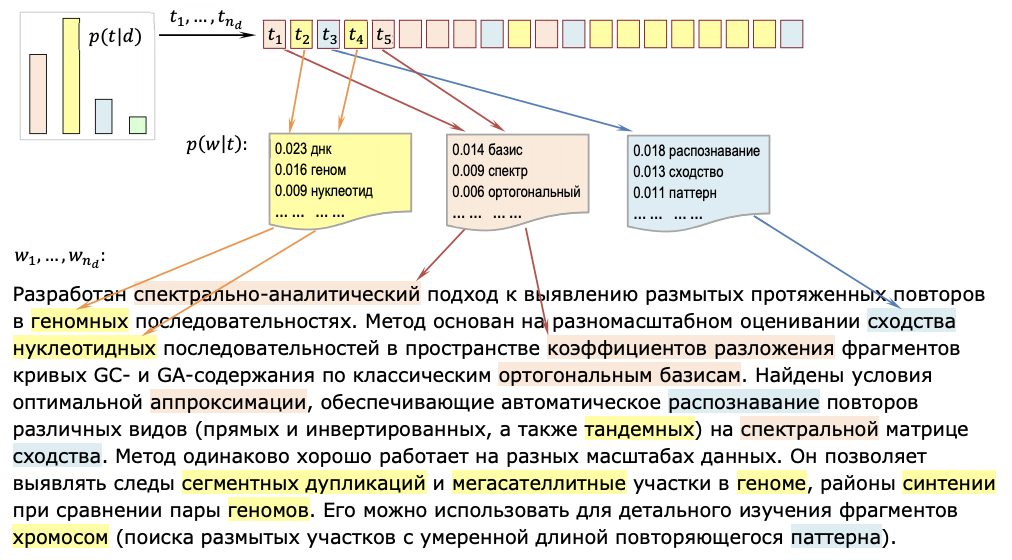
\includegraphics[width=0.9\linewidth]{../resources/a1.png}}
\caption{Процесс порождения текстового документа вероятностной тематической моделью}
\label{ris:a1}
\end{figure}
   
   Построение тематической модели --- это обратная задача: по известной коллекции $D$ требуется восстановить породившие её распределения $p(t| d)$ и $p(w |t)$.
   
  \textbf{Дано:}  коллекция текстовых документов
  
     \begin{itemize} 
\item $n_{dw}$ --- частоты терминов в документах, $\hat{p}(w|d)=\frac{n_{dw}}{n_d}$
\end{itemize}
   
   \newpage
   
  \textbf{Найти:} параметры тематической модели $p(w|d)=\sum_{t\in T}\phiup_{wt}\thetaup_{td}$
   
      \begin{itemize} 
\item $\phiup_{wt}=p(w|t)$ --- вероятности терминов $w$ в каждой теме $t$
\item $\thetaup_{td}=p(t|d)$ --- вероятности тем $t$ в каждом документе $d$
\end{itemize}  
  
  Это задача стохастического матричного разложения:
  
     \begin{figure}[!h]
\center{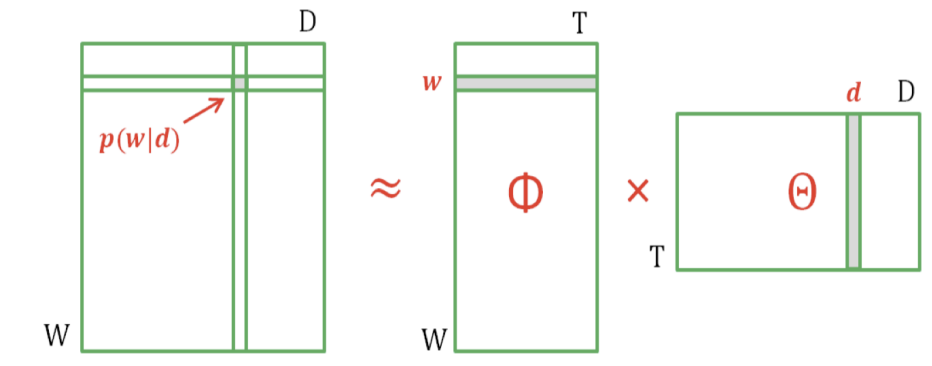
\includegraphics[width=0.7\linewidth]{../resources/a2.png}}
\caption{Задача стохастического матричного разложения}
\label{ris:a1}
\end{figure}
  
  Если $\mathbf{\Phi}$ и $\mathbf{\Theta}$ --- решение, то
	    существует матрица $\mathbf{S}$ ранга $|T|$ такая, что $\mathbf{\Phi}^{'}\mathbf{\Theta}^{'} = (\mathbf{\Phi} \mathbf{S})(\mathbf{S}^{-1}\mathbf{\Theta})$, но $\mathbf{\Phi}^{'}$ и $\mathbf{\Theta}^{'}$ не обязательно стохастические, т.е. метод главных компонент не подходит для тематического моделирования.
  
  
  %Здесь возникает ряд проблем, потому что мы знаем вот что есть анализ главных компонент и мы можем на самом деле найти k главных компонент и казалось бы задача решена. но неправда т.к. решение не единственно (типа факторный анализ, можно вращать), все-равно получим тот же результат
 % а также можем наткнуться на то, что наши новые матрицы не обызательно стохастическими будут. Если мы запишем метод наименьших квадратов, то можем как раз наткнуться на проблему, что мы получим матрицы, которые не будут являться стохастическими. А это основное условие т.к. имеем дело с вероятностями
  
 % Если не про стохастичность, а про единственность, то в принципе если нам важно, чтоб первое было самым важным (важна упорядоченность, то фиксировано одно решение) А если не важна упорядоченность просто есть набор равноценных тем и тогда неоднозначно решение т.к. упорядоченность не важна.
  
  
  
 \subsection{Частотные оценки условных вероятностей} 
 
 Вероятности, связанные с наблюдаемыми переменными $d$ и $w$, можно оценивать по выборке как частоты (здесь и далее
выборочные оценки вероятностей $p$ будем обозначать через $\hat{p}$):
 
 \[
 \hat{p}(d, w) = \frac{n_{d w}}{n}, \;\;\; \hat{p}(d) = \frac{n_d}{n}, \;\;\; \hat{p}(w) = \frac{n_{w}}{n}, \;\;\; \hat{p}(w, d) = \frac{n_{d w}}{n_d},\;\; \text{ где}
 \]
  
   \begin{itemize}
       \item $n_{d w}$ --- число вхождений термина $w$ в документ $d$;
       \item $n_d = \sum_{w \in W} n_{d w}$ --- длина документа $d$ в терминах;
       \item $n_w = \sum_{d \in D}n_{d w}$ --- число вхождений термина $w$ во все документы коллекции;
       \item $n = \sum_{d \in D} \sum_{w \in W} n_{dw}$ --- длина коллекции $d$ в терминах.
       \end{itemize}
       
 
 Вероятности, связанные со скрытой переменной $t$, также можно оценивать как частоты, если рассматривать коллекцию документов как выборку троек $(d, w, t)$:      
 
  \[
  \hat{p}(t) = \frac{n_t}{n}, \;\;\; \hat{p}(w|t) = \frac{n_{w t}}{n_t}  \;\;\; \hat{p}(t|d) = \frac{n_{d t}}{n_d} \;\;\; \hat{p}(t|d, w) = \frac{n_{d w t}}{n_{d w}},\;\; \text{ где}
  \]
  
   \begin{itemize}
       \item $n_{d w t}$ --- число троек, в которых термин $w$ в документе $d$ связан с темой $t$;
       \item $n_{d t} = \sum_{w \in W} n_{d w t}$ --- число троек, в которых термин в документе $d$ связан с темой $t$;
       \item $n_{w t} = \sum_{d \in D} n_{d w t}$ --- число троек, в которых термин $w$ связан с темой~$t$;
       \item $n_t = \sum_{d \in D} \sum_{w \in W} n_{d w t}$ --- число троек, связанных с темой $t$.
   \end{itemize}
 
 В пределе $n \to \infty$ частотные оценки $\hat{p}(\cdot)$ стремятся к соответствующим вероятностям $p(\cdot)$, согласно закону больших чисел.

Частотная интерпретация даёт ясное понимание всех условных вероятностей, которые будут использоваться в дальнейшем.
  
  
  
   \section{Вероятностный латентный семантический анализ PLSA} 
  
   \subsection{Стохастическое матричное разложение} 
  
  Если число тем $|T|$ много меньше числа документов $|D|$ и числа терминов $|W|$, то равенство $p(w|d)=\sum_{t\in T}p(t|d)p(w|t)$  можно понимать как задачу
приближённого представления заданной матрицы частот:

\[
F=(\hat{p}_{wd})_{W\times D},\;\;\;\hat{p}_{wd}=\hat{p}(w|d)=\frac{n_{dw}}{n_d},
\]
  
  
в виде произведения $\mathbf{F}\approx\mathbf{\Phi}\mathbf{\Theta}$ двух неизвестных матриц меньшего размера — матрицы терминов тем $\mathbf{\Phi}$ и матрицы тем документов $\mathbf{\Theta}$, где


    \begin{equation*}
\begin{gathered}
   \mathbf{\Phi} = (\phi_{wt})_{W \times T},\;\;\; \phi_{w t} = p(w|t);\\ \mathbf{\Theta} = (\theta_{td})_{T \times D},\;\;\; \theta_{t d} = p(t|d).
   \end{gathered}
\end{equation}
  
  
Матрицы, столбцы которых неотрицательны и нормированы, следовательно, могут пониматься как дискретные распределения, называются стохастическими.


В вероятностном тематическом моделировании вместо принципа наименьших квадратов используется принцип максимума правдоподобия.
  
   
      \subsection{Принцип максимума правдоподобия} 
      
  Для оценивания параметров $\mathbf{\Phi}$, $\mathbf{\Theta}$ тематической модели по коллекции документов $D$ будем максимизировать плотность распределения выборки:
  
  \[
  p(D,\mathbf{\Phi},\mathbf{\Theta})=C\prod_{d\in D}\prod_{w\in d}p(d,w)^{n_{dw}}=\prod_{d\in D}\prod_{w\in d}p(w|d)^{n_{dw}}\underbrace{Cp(d)^{n_{dw}}}_{const}\to \max_{\mathbf{\Phi},\mathbf{\Theta}},\;\;\text{где}
  \]
      
  где $C$ --- нормировочный множитель, зависящий только от чисел $n_{dw}$. Отбросим множители $C $и $p(d)$, не влияющие на положение точки максимума, подставим выражение для $p(w | d)$. Прологарифмируем $p(D; \mathbf{\Phi},\mathbf{\Theta})$, чтобы превратить произведения в суммы. Получим задачу максимизации логарифма правдоподобия при ограничениях
неотрицательности и нормированности столбцов матриц $\mathbf{\Phi}$ и $\mathbf{\Theta}$:    
      
      \begin{gather*}
        \begin{cases}
        \mathcal{L}_{\log}(\mathbf{\Phi}, \mathbf{\Theta}) = \sum\limits_{d \in D} \sum\limits_{w \in d} n_{d w} \ln{\sum\limits_{t \in T} \phi_{w t} \theta_{t d}} \to \max\limits_{\mathbf{\Phi}\mathbf{\Theta}}\\
        \phi_{w t} \geq 0,\;\;\; \sum\limits_{w \in W} \phi_{w t} = 1\\
        \theta_{t d} \geq 0,\;\;\; \sum\limits_{t \in T}\theta_{t d} = 1.
        \end{cases}
     \end{gather*}
      
     Для решения задачи применяется ЕМ-алгоритм 
      
    
      \subsection{EM-алгоритм} 
      
      Для решения задачи в PLSA применяется итерационный процесс, в котором каждая итерация состоит из двух шагов — Е (expectation) и М (maximization).

Перед первой итерацией выбирается начальное приближение параметров $\phi_{w t}$, $\theta_{t d}$.
      
     
     \textbf{Е-шаг.}
     
     На E-шаге по текущим значениям параметров $\phi_{w t}$, $\theta_{t d}$ с помощью формулы Байеса вычисляются условные вероятности $p(t| d, w)$ всех тем $t \in T$ для каждого
термина $w\in d$ в каждом документе $d$:

\[
 H_{d w t} = p(t|d, w) = \frac{p(w|t) p(t|d)}{p(w|d)} = \frac{\phi_{w t} \theta_{t d}}{\sum_{s \in T} \phi_{w s} \theta_{s d}}.
\]

\textbf{M-шаг.}

На M-шаге, наоборот, по условным вероятностям тем $H_{d w t}$ вычисляется новое приближение параметров $\phi_{w t}$, $\theta_{t d}$. Это легко сделать, если заметить, что величина

\[
\hat{n}_{dwt}=n_{dw}p(t|d,w)=n_{dw}H_{dwt}
\]

оценивает (не обязательно целое) число $n_{dwt}$ вхождений термина $w$ в документ $d$, связанных с темой $t$. Просуммировав $\hat{n}_{dwt}$ по документам $d$ и по терминам $w$, получим оценки $\hat{n}_{wt}$, $\hat{n}_{dt}$, $\hat{n}_{t}$
, и через них --- частотные оценки условных вероятностей $\phi_{w t}$, $\theta_{t d}$:

\begin{gather*}
    \phi_{w t} = \frac{\hat{n}_{w t}}{\hat{n}_t}, \;\;\; \hat{n}_{w t} = \sum_{d \in D}n_{d w} H_{d w t}, \;\;\;  \hat{n}_t = \sum_{w \in W}\hat{n}_{w t};\\
    \theta_{t d} = \frac{\hat{n}_{d t}}{\hat{n}_d}, \;\;\;  \hat{n}_{d t} = \sum_{w \in d} n_{d w} H_{d w t}, \;\;\;  \hat{n}_d = \sum_{t \in T} \hat{n}_{d t}.
\end{gather*}

Покажем теперь, что эти оценки действительно являются решением задачи максимизации правдоподобия при фиксированных $H_{dwt}$:

Запишем лагранжиан задачи максимизации логарифма правдоподобия при ограничениях нормировки, проигнорировав ограничения неотрицательности:

\[
\mathcal{L}(\mathbf{\Phi}, \mathbf{\Theta}) = \sum\limits_{d \in D} \sum\limits_{w \in d} n_{d w} \ln{\underbrace{\sum\limits_{t \in T} \phi_{w t} \theta_{t d}}_{p(w|d)}} - \sum_{t\in T}\lambda_t(\sum_{w\in W}\phi_{wt}-1)-\sum_{d\in D}\mu_d(\sum_{t\in T}\theta_{td}-1).
\]

Продифференцировав лагранжиан по $\phi_{wt}$ и приравняв нулю производную, получим

\[
\lambda_t=\sum_{d\in D}n_{dw}\frac{\theta_{td}}{p(w|d)}
\]

Домножим обе части этого равенства на $\phi_{wt}$, просуммируем по всем терминам $w\in W$, применим условие нормировки вероятностей $\phi_{wt}$ в левой части и выделим переменную $H_{dwt}$ в правой части. Получим

\[
\lambda_t=\sum_{d\in D}\sum_{w\in W}n_{dw}H_{dwt}
\]

Снова домножим обе части на $\phi_{wt}$, выделим переменную $H_{dwt}$ в правой части и выразим $\phi_{wt}$ из левой части, подставив уже известное выражение для $\lambda_t$. Получим

\[
\phi_{wt}=\frac{\sum_{d\in D}n_{dw}H_{dwt}}{\sum_{w^{'}\in W}\sum_{d\in D}n_{dw^{'}}H_{dw^{'}t}}
\]

Обозначив числитель через $\hat{n}_{wt}$, получим

\[
\phi_{w t} = \frac{\hat{n}_{w t}}{\hat{n}_t}, \;\;\; \hat{n}_{w t} = \sum_{d \in D}n_{d w} H_{d w t}, \;\;\;  \hat{n}_t = \sum_{w \in W}\hat{n}_{w t}
\]

Проделав аналогичные действия
с производной лагранжиана по \theta_{t d}, получим 

\[
\theta_{t d} = \frac{\hat{n}_{d t}}{\hat{n}_d}, \;\;\;  \hat{n}_{d t} = \sum_{w \in d} n_{d w} H_{d w t}, \;\;\;  \hat{n}_d = \sum_{t \in T} \hat{n}_{d t}
\]

Заметим, что если начальные приближения $\theta_{t d}$ и $\phi_{w t}$ положительны, то и после каждой итерации они будут оставаться положительными, несмотря на то, что ограничение неотрицательности было проигнорировано в ходе решения.



\subsection{Начальное приближение $\phi_{w t}$ и $\theta_{t d}$} 

Начальное приближение можно задать нормированными случайными векторами из равномерного распределения. 

Другая распространённая рекомендация --- пройти по всей коллекции, выбрать для каждой пары $(d, w)$ случайную тему $t$, вычислить частотные оценки вероятностей $\phi_{w t}$ и $\theta_{t d}$ для всех $d\in D$, $w\in W$, $t\in T$.


\textbf{Инициализация с частичным обучением} (некоторые $t$ известны заранее и имеются дополнительные данные о привязке некоторых $d$ или $w$ к $t$):
    \begin{itemize}
        \item Если известно, что документ $d$ относится к подмножеству $T_d \subset T$, то в качестве начального $\theta_{t d}$ можно взять равномерное распределение на этом подмножестве:
        
        \begin{gather*}
            \theta_{t d}^0 = \frac{1}{|T_d|}[t\in T_d].
        \end{gather*}
        
        \item Если известно, что подмножество терминов $W_t \subset W$ относится к теме $t$, то в качестве начального $\phi_{w t}$ можно взять равномерное распределение на $W_t$:
        
            \begin{gather*}
            \phi_{wt}^0 = \frac{1}{|W_t|}[w\in W_t].
        \end{gather*}
        
        \item Если известно, что некоторое подмножество документов $D_t \subset D$ относится к теме $t$,то можно взять эмпирическое распределение слов в объединённом документе:

        \begin{gather*}
        \phi_{wt}^0 = \frac{\sum_{d \in D} n_{d w}}{\sum_{d \in D_t} n_d}.
        \end{gather*}
        
        \item Если нет никакой априорной информации о связи документов с темами, то последнюю формулу можно применить к случайным подмножествам документов $D_t$.
    \end{itemize}
    
   \subsection{Недостатки PLSA}  
    
    У PLSA существуют некоторые недостатки, рассмотрим их:
    
  \begin{enumerate}
    \item Медленно сходится на больших коллекциях, так как $\mathbf{\Phi}$ и $\mathbf{\Theta}$ обновляются после каждого прохода коллекции.
    
    
    \item Не разреживает распределение $H_{d w t} = p(t| d, w)$.
    
    
    \item Вынуждены хранить матрицу $\mathbf{H} = (H_{d w t})_{D \times W \times T}$.
    
    
    \item Слишком много параметров $\phi_{w t}$ и $\theta_{t d}$ ($|W||T| + |T||D|)$.
    
    
    \item Неверно оценивает вероятность новых слов ($\hat{p}(w|t) = 0$ для слова, которого не было в обучающейся коллекции, но оно встретилось в каком-нибудь документе).
    
    
    \item Не позволяет управлять разреженностью $\mathbf{\Phi}$ и $\mathbf{\Theta}$:
    \begin{gather*}
        (\text{в начале } \phi_{w t} = 0) \Leftrightarrow  (\text{в конце }  \phi_{w t} = 0),\\
         (\text{в начале }  \theta_{t d} = 0) \Leftrightarrow  (\text{в конце } \theta_{t d} = 0).
    \end{gather*}
\end{enumerate}
    
     \subsection{Модификации}  
     
     Как мы увидели, у алгоритма существует достаточно много недостатков, поэтому чаще используют модификации метода, которые помогают устранить некоторые из них.
     
     
     
     
     
     \subsubsection{Рациональный EM–алгоритм}  
     
     \textbf{Проблема:} Вынуждены хранить матрицу $\mathbf{H} = (H_{d w t})_{D \times W \times T}$.


\textbf{Решение:} Вычислять $H_{d w t}$ по мере необходимости.

\textbf{Обоснование}:

     Вычисление переменных $\hat{n}_{wt}$, $\hat{n}_{dt}$, $\hat{n}_{t}$ на М-шаге требует однократного прохода всей коллекции в цикле по всем документам $d\in D$ и всем
терминам $w\in d$. Внутри этого цикла переменные $H_{dwt}$ можно вычислять непосредственно в тот момент, когда они понадобятся. От этого результат алгоритма не изменяется, Е-шаг встраивается внутрь M-шага без дополнительных вычислительных затрат, отпадает необходимость хранения трёхмерной матрицы $H_{dwt}$. Заметим также,
что переменную $\hat{n}_d$ можно не вычислять, поскольку $\hat{n}_d=n_d$.
     


     \begin{algorithm}[H]
\begin{algorithmic}[1]
\REQUIRE Коллекция $D$, число тем $T$, начальные $\mathbf{\Phi}$ и $\mathbf{\Theta}$
\ENSURE Распределения $\mathbf{\Phi}$ и $\mathbf{\Theta}$
\REPEAT
\STATE обнулить $\hat{n}_{w t}, \hat{n}_{d t}, \hat{n}_t$ для всех $d \in D$, $w \in W$, $t \in T$;
\FORALL{$d \in D$, $w \in d$}
\STATE $Z:=\sum_{t \in T} \phi_{w t} \theta_{t d}$;
\FORALL{$t \in T$ таких, что $\phi_{w t} \theta_{t d} > 0$}
\STATE увеличить $\hat{n}_{w t}, \hat{n}_{d t}, \hat{n}_t$ на $\frac{n_{d w}}{Z}\phi_{w t} \theta_{t d}$;
\ENDFOR
\ENDFOR\\

$\phi_{w t} := \hat{n}_{w t}/\hat{n}_t$ для всех $w \in W$, $t \in T$;\\
$\theta_{t d} := \hat{n}_{d t}/n_d$ для всех $d \in D$, $t \in T$;
\UNTIL{$\mathbf{\Phi}$ и $\mathbf{\Theta}$ не стабилизируются;}
\end{algorithmic}
\caption{Рациональный ЕМ-алгоритм}
\label{alg:seq}
\end{algorithm}
     
     
     
    
     
     \subsubsection{Обобщенный ЕM-алгоритм}  

\textbf{Проблема:}{PLSA медленно сходится на больших коллекциях.}


\textbf{Решение:} Обновлять значения $\mathbf{\Phi}$ и $\mathbf{\Theta}$ чаще.

\textbf{Обоснование}:

В ЕМ-алгоритме нет необходимости сверхточно решать задачу максимизации правдоподобия на M-шаге. Достаточно ещё немного приблизиться к точке максимума правдоподобия и снова выполнить E-шаг. Это связано с тем, что сам функционал правдоподобия известен не точно --- он зависит от приближённых значений $H_{dwt}$,
полученных на Е-шаге. Другое обобщение состоит в том, что E-шаг выполняется только для части скрытых переменных $H_{dwt}$. После этого M-шаг выполняется только для тех основных переменных $\phi_{wt}$, $\theta_{td}$, которые зависят от изменившихся скрытых переменных. 

В случае PLSA сокращение M-шага сводится к более частому обновлению параметров $\phi_{wt}$ и $\theta_{td}$ по значениям счётчиков $\hat{n}_{wt}$ и $\hat{n}_{dt}$. Частота обновления выбирается --- после каждого документа, термина, и т.д. 

На больших коллекциях частые обновления повышают скорость сходимости. Частота обновления влияет на скорость сходимости и почти не влияет на значение правдоподобия в конце итераций. Отсюда следует практическая рекомендация делать обновления после каждого термина, при этом каждый термин документа обрабатывается только один раз. Этот способ имеет дополнительное преимущество --- внутри алгоритма можно отказаться от хранения матриц $\mathbf{\Phi}$ и $\mathbf{\Theta}$. Обновления после каждого вхождения термина являются избыточно частыми, в этом случае каждый термин документа приходится обрабатывать $n_{dw}$ раз.

Необходимость хранения трёхмерной матрицы $n_{dwt}$ делает алгоритм неприменимым к большим коллекциям. Этот недостаток можно устранить, например, сэмплированием. 

\begin{algorithm}[H]
\begin{algorithmic}[1]
\REQUIRE Коллекция $D$, число тем $T$, начальные $\mathbf{\Phi}$ и $\mathbf{\Theta}$
\ENSURE Распределения $\mathbf{\Phi}$ и $\mathbf{\Theta}$\\
\STATE Обнулить $\hat{n}_{w t}, \hat{n}_{d t}, \hat{n}_t$, $\hat{n}_d$, $\hat{n}_{d w t}$ для всех $d \in D$, $w \in W$, $t \in T$;
\REPEAT
\FORALL{$d \in D$, $w \in d$}
\STATE $Z:=\sum_{t \in T} \phi_{w t} \theta_{t d}$;
\FORALL{$t \in T$ таких, что $n_{d w t} > 0$ или $\phi_{w t} \theta_{t d} > 0$}
\STATE увеличить $\hat{n}_{w t}$, $\hat{n}_{d t}$, $\hat{n}_t$, $\hat{n}_d$ на $\frac{n_{d w}}{Z}\phi_{w t} \theta_{t d} - n_{d w t}$;\\
$n_{d w t} := \frac{n_{d w}}{Z} \phi_{w t} \theta_{t d} - n_{d w t}$;
\ENDFOR
\IF{не первая итерация и пора обновить параметры $\mathbf{\Phi}$ и $\mathbf{\Theta}$}
\STATE $\phi_{w t} := \hat{n}_{w t}/\hat{n}_t$ для всех $w \in W$, $t \in T$ таких, что $\hat{n}_{w t}$ изменился;\\

$\theta_{t d} := \hat{n_{d t}}/\hat{n}_d$ для всех $d \in D$, $t\in T$ таких, что $\hat{n}_{t d}$ изменился;
\ENDIF
\ENDFOR
\UNTIL{$\mathbf{\Phi}$ и $\mathbf{\Theta}$ не стабилизируются;}
\end{algorithmic}
\caption{Обобщенный ЕМ-алгоритм}
\label{alg:seq}
\end{algorithm}

   \subsubsection{Модификация обобщенного ЕM-алгоритма}  

\textbf{Проблема:} Необходимо хранить массив $n_{d w t} = n_{d w} H_{ d w t}$, который занимает $O(n|T|)$ памяти.

\textbf{Решение:} На М-шаге вместо распределения $H_{d w t} \equiv p(t|d, w)$ взять его несмещенную эмпирическую оценку по очень маленькой выборке длины $s$:

\begin{gather*}
\hat{H}_{d w t} = \hat{p}(t| d, w) = \frac{1}{s}\sum\limits_{i=1}^s \mathbb{I}_{t_{d w i} = t}.
\end{gather*}

В ряде публикаций предложено экономное сэмплирование, когда $s$ уменьшается до 3–5 тем,что приводит к большему разреживанию и экономии вычислительных ресурсов без существенной потери качества тематической модели.


 





\nocite{*}
 


 


\end{document} 